\chapter{Experimentos}

En capítulos anteriores se han expuesto los objetivos marcados para la realización del proyecto así como la solución desarrollada para cada uno de estos problemas y las herramientas utilizadas para los mismos. En este capítulo se muestran los experimentos que se han ido realizando según íbamos cumpliendo objetivos y que sirven como validación experimental de la solución programada.\\

\section{Experimentos con simulador Gazebo}

Una vez desarrollado el proyecto y satisfaciendo todos los objetivos marcados se han realizado pruebas sobre la el drone simulado en Gazebo para comprobar sin ningún tipo de riesgos el funcionamiento del mismo.\\

Para realizar este experimento asemejandose de la manera más realista al experimento final con el drone real se ha utilizado un \emph{Intel Compute Stick}\footnote{\url{http://www.intel.com/content/www/us/en/compute-stick/compute-stick-product-brief.html}} como par local, encargado de conectarse a las interfaces ICE que nos proporciona el plugin ArDrone desarrollado por JdeRobot para el simulador Gazebo. Este ordenador está compuesto por un procesador Intel Atom que corre Ubuntu 14.04 LTS como sistema operativo. El simulador Gazebo se ha ejecutado en un portátil auxiliar y utilizaremos otro equipo portátil como par remoto desde el que teleoperaremos el drone además de ejecutar el servidor de señalización. La figura \ref{fig:esquemaexperimento1} muestra el esquema del montaje de este experimento. \\

\begin{figure}[h!]
\centering
\includegraphics[width=0.9\textwidth]{experimento1}
\caption{Esquema del experimento con el simulador gazebo.}
\label{fig:esquemaexperimento1}
\end{figure}

Los resultados de este experimento han sido muy positivos, el control y manejo del drone ha sido de manera fluida y sin realizar ningún tipo de movimiento extraño producido por algún tipo de mal-funcionamiento del código. El manejo se ha realizado tanto con los \emph{joysticks} virtuales como con el mando. Puedes ver un fotograma del vídeo\footnote{\url{http://jderobot.org/Irodmar-tfg#WebRTC_on_a_drone_working_with_Gazebo5}} del experimento en la figura \ref{fig:experimentogazebo}.\\

\begin{figure}[h!]
\centering
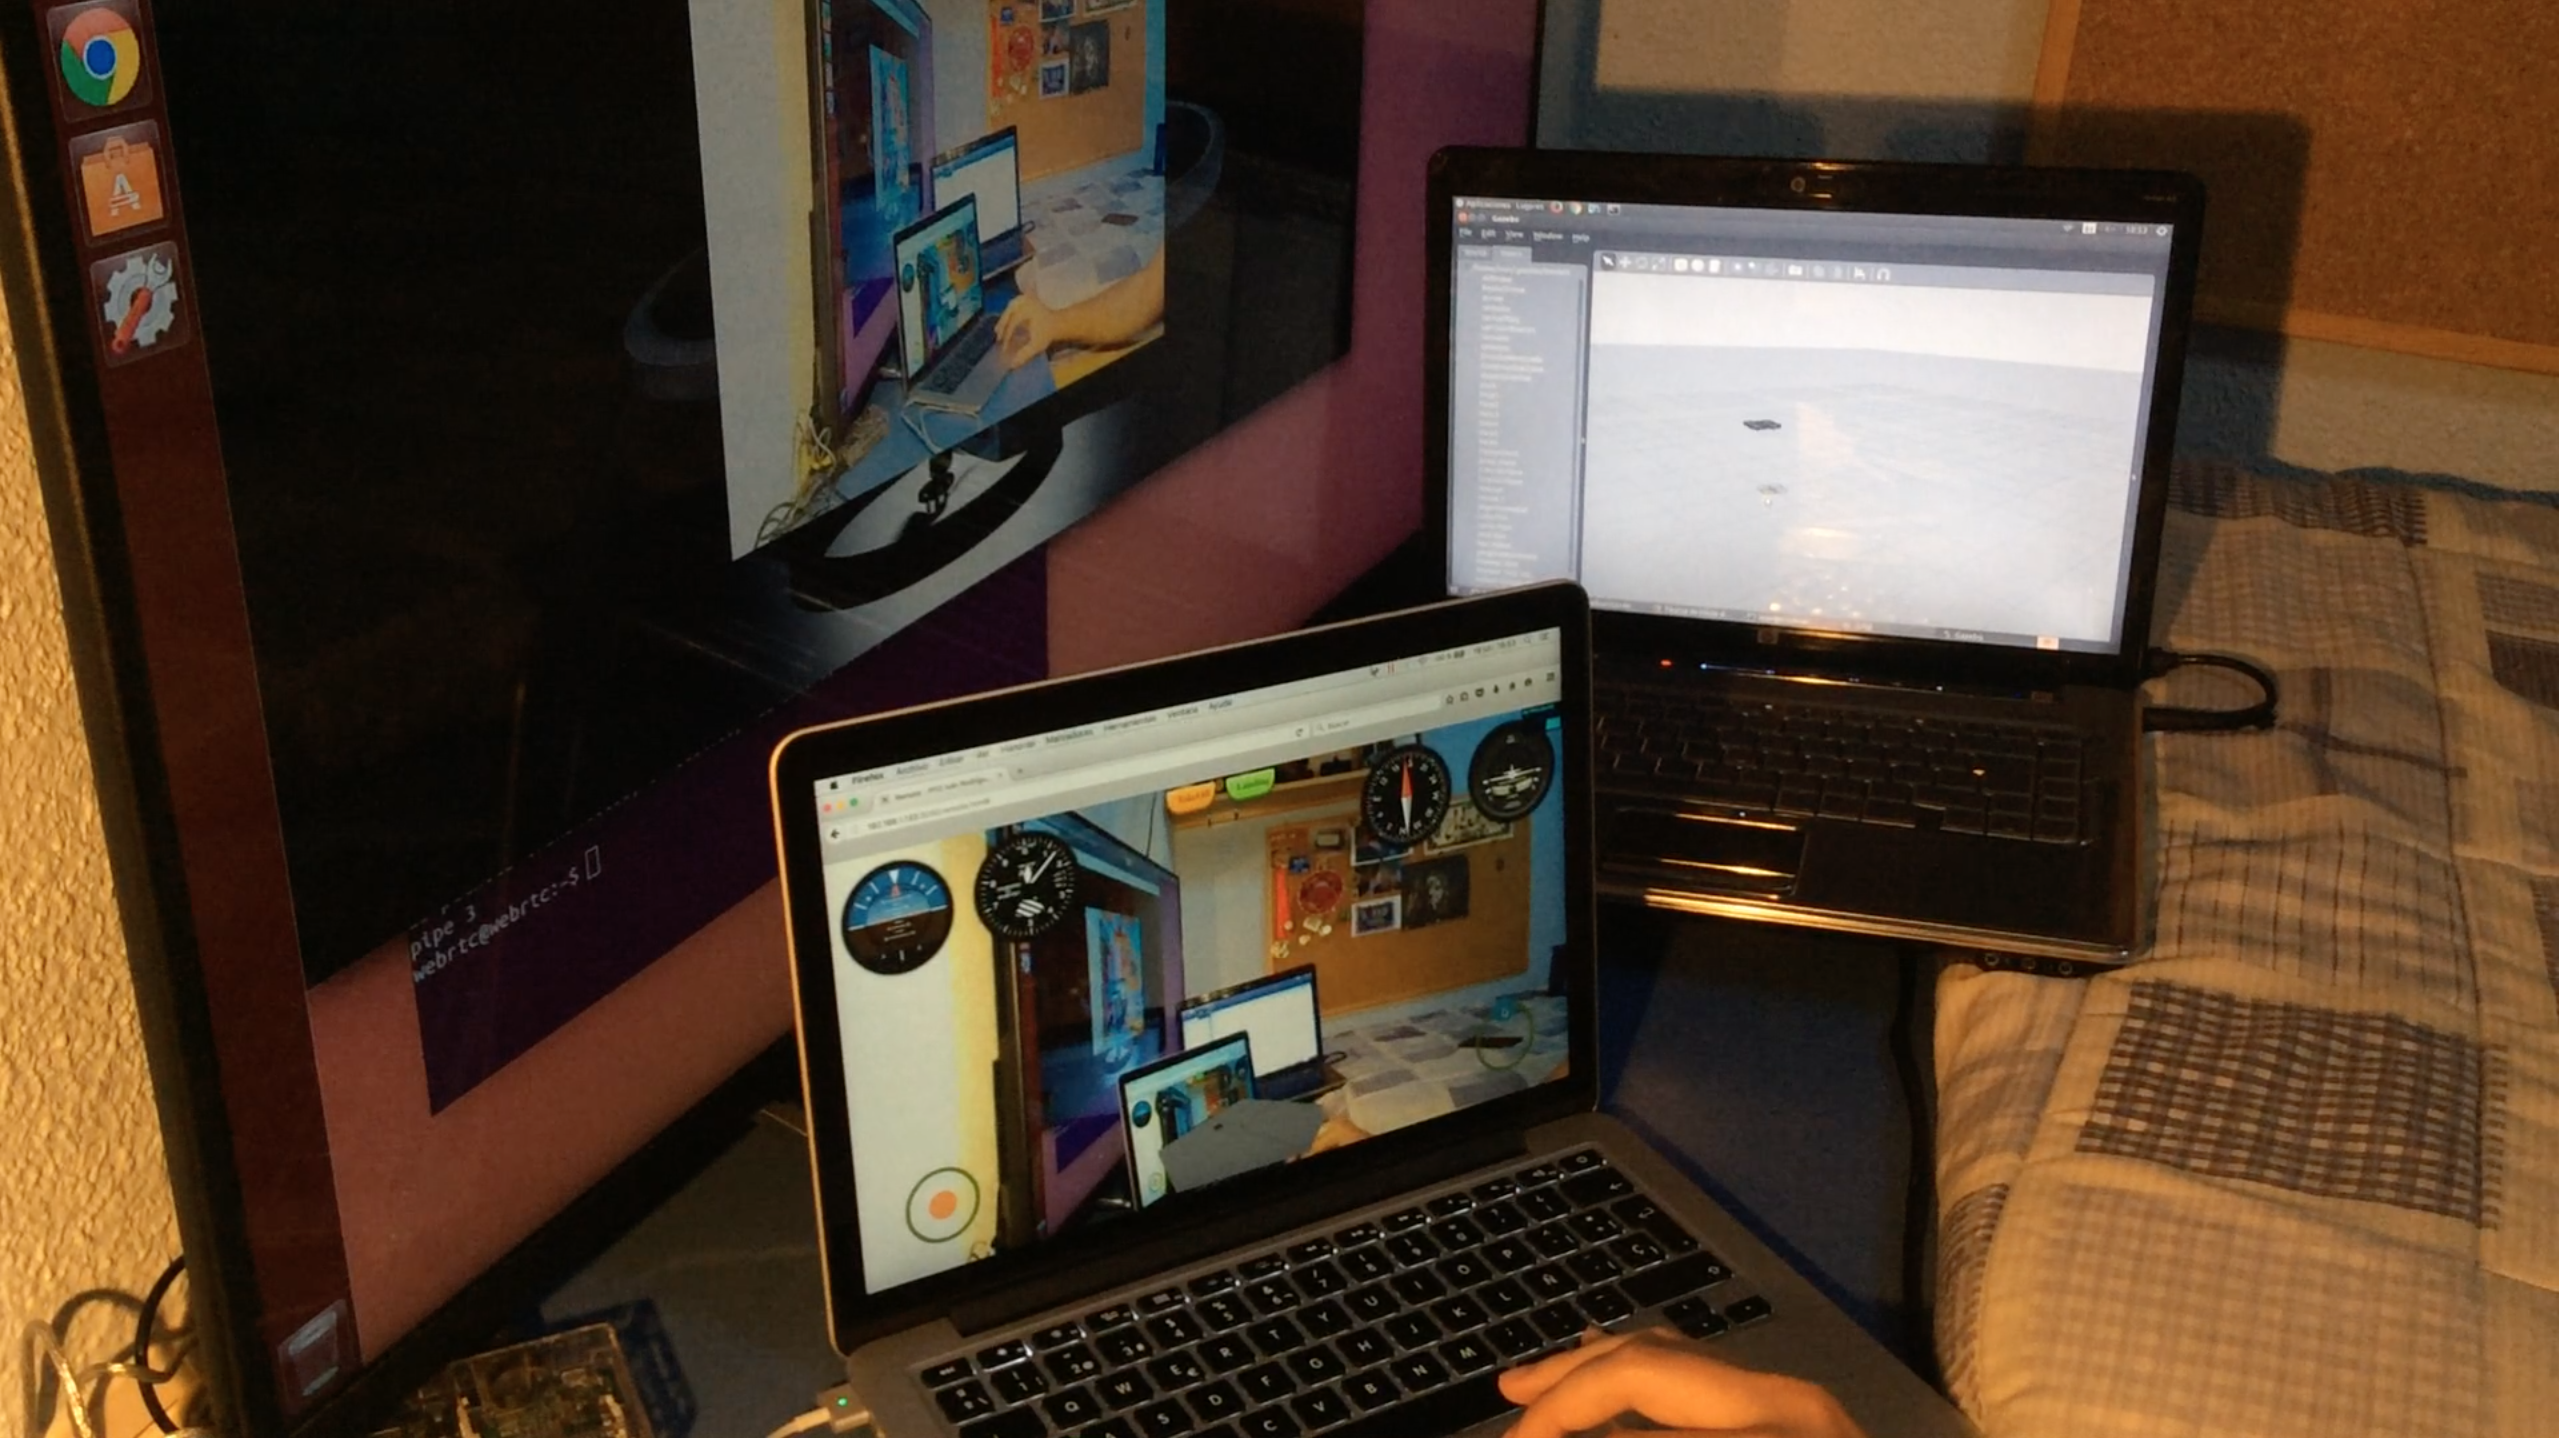
\includegraphics[width=0.9\textwidth]{experimentogazebo}
\caption{Experimento con el simulador gazebo.}
\label{fig:experimentogazebo}
\end{figure}

En la siguiente figura (\ref{fig:secexp1}) se puede observar la secuencia de movimiento del drone durante el experimento.\\
\newpage
\begin{figure}[h!]
\centering
  \begin{subfigure}[]{47mm}
    \includegraphics[width=47mm]{sec_exp1_1}
  \end{subfigure}
  \hspace{0.5pt}
  \begin{subfigure}[]{47mm}
    \includegraphics[width=47mm]{sec_exp1_2}
  \end{subfigure}
    \hspace{0.5pt}
    \begin{subfigure}[]{47mm}
    \includegraphics[width=47mm]{sec_exp1_3}
  \end{subfigure}
    \caption{Secuencia de movimiento del experimento con Gazebo.}
  \label{fig:secexp1}
\end{figure}

Una vez superado este experimento se ha realizado el siguiente, consistiendo en realizar pruebas con el drone real.\\

\section{Vuelo del drone real}

Las pruebas con el drone real se han divido a su vez en dos. La primera consiste en realizar las pruebas sin colocar a bordo del drone ni el \emph{computer stick} ni la cámara. Ambos se han usado para las pruebas pero para una primera aproximación se han realizado sin estar a bordo.\\

Así pues la distribución de los equipos es: computer stick como par local, que se conecta al drone real y accede a la cámara USB conectada al mismo, y ordenador portátil como par remoto desde el que se teleoperará el drone y a su vez está ejecutando el servidor de señalización y el \texttt{ardrone\_server.} La figura \ref{fig:experimentodronereal1} muestra la realización de este experimento. En la mediawiki\footnote{\url{http://jderobot.org/Irodmar-tfg\#First\_Flying\_with\_Real\_Drone}}\cite{Mediawiki} hay un vídeo completo del mismo.\\

\begin{figure}[h!]
\centering
\includegraphics[width=0.9\textwidth]{experimentodronereal1}
\caption{Experimento uno con drone real.}
\label{fig:experimentodronereal1}
\end{figure}


\begin{figure}[h!]
\centering
  \begin{subfigure}[]{48mm}
    \includegraphics[width=48mm]{sec_exp2_1}
  \end{subfigure}
  \hspace{1pt}
  \begin{subfigure}[]{48mm}
    \includegraphics[width=48mm]{sec_exp2_2}
  \end{subfigure}
    \hspace{1pt}
    \begin{subfigure}[]{48mm}
    \includegraphics[width=48mm]{sec_exp2_3}
  \end{subfigure}
    \caption{Secuencia de movimiento del experimento con el drone real.}
  \label{fig:secexp2}
\end{figure}


Esta prueba también ha sido un éxito, por lo que nos marcamos el siguiente experimento con el drone y la cámara a bordo del drone. Este experimento la configuración es la misma que en el anterior, pero el manejo del drone con la aplicación será más realista ya que tenemos la cámara en primera persona.\\

La configuración de los equipos en este experimento ha consistido en colocar a bordo del drone la cámara, el \emph{computer stick}, el cuál actuará como par local, estableciendo la conexión con el drone y accediendo a la cámara. El drone tiene una conexion USB de salida pero la potencia no es suficiente para hacer funcionar el \emph{computer stick}. Por este motivo se ha tenido que colocar a bordo una pila la cual hará las veces de fuente de alimentación. Por otro lado tenemos un ordenador el cual actúa como par remoto desde el que teleoperaremos el drone y ademas se ha utilizado para ejecutar tanto el servidor de señalizacion como el servidor \emph{ardrone\_server}.\\

Este experimento ha sido fallido únicamente por las capacidades de vuelo que nos ofrece el drone. Entre los dispositivos que hemos colocado a bordo superamos la carga máxima de pago que permite este cuadricóptero. En lo que al desarrollo se refiere ha funcionado perfectamente ya que en el par remoto obteníamos las imágenes y datos de vuelo procedentes del drone, y al ejecutar lar orden de despegue el cuadricóptero ha intentado levantar el vuelo sin conseguirlo.\\

*** FIN EXPERIMENTO CON FOTO Y LINK AL VIDEO***


\section{Vuelos con multidispositivos}

Como tercer y último experimento hemos probado a volar el drone utilizando dispositivos móviles. WebRTC tiene soporte para dispositivos móviles y los elementos de control los hemos desarrollado también para dispositivos táctiles, podemos utilizarlos como par remoto, par local o ambos. Al igual que el experimento anterior se ha realizado en dos pasos, primero sin colocar el dispositivo a bordo del drone para confirmar su correcto funcionamiento y posteriormente repitiéndolo con el dispositivo a bordo. Realizar experimentos con dispositivos móviles implica la necesidad de la utilización de un ordenador de apoyo que será el que ejecute tanto el servidor de señalización para WebRTC cómo \emph{ardrone\_server}.\\

Como primer experimento se ha utilizado un ordenador como par local y un móvil como par remoto desde el que gobernamos los movimientos del drone. En la figura \ref{fig:experimentodronemultidispositivo1} se puede apreciar un instante del experimento cuyo vídeo se encuentra en la mediawiki\footnote{\url{http://jderobot.org/Irodmar-tfg\#Flying\_with\_a\_mobile\_like\_Remote\_PC}}.\\

\begin{figure}[h!]
\centering
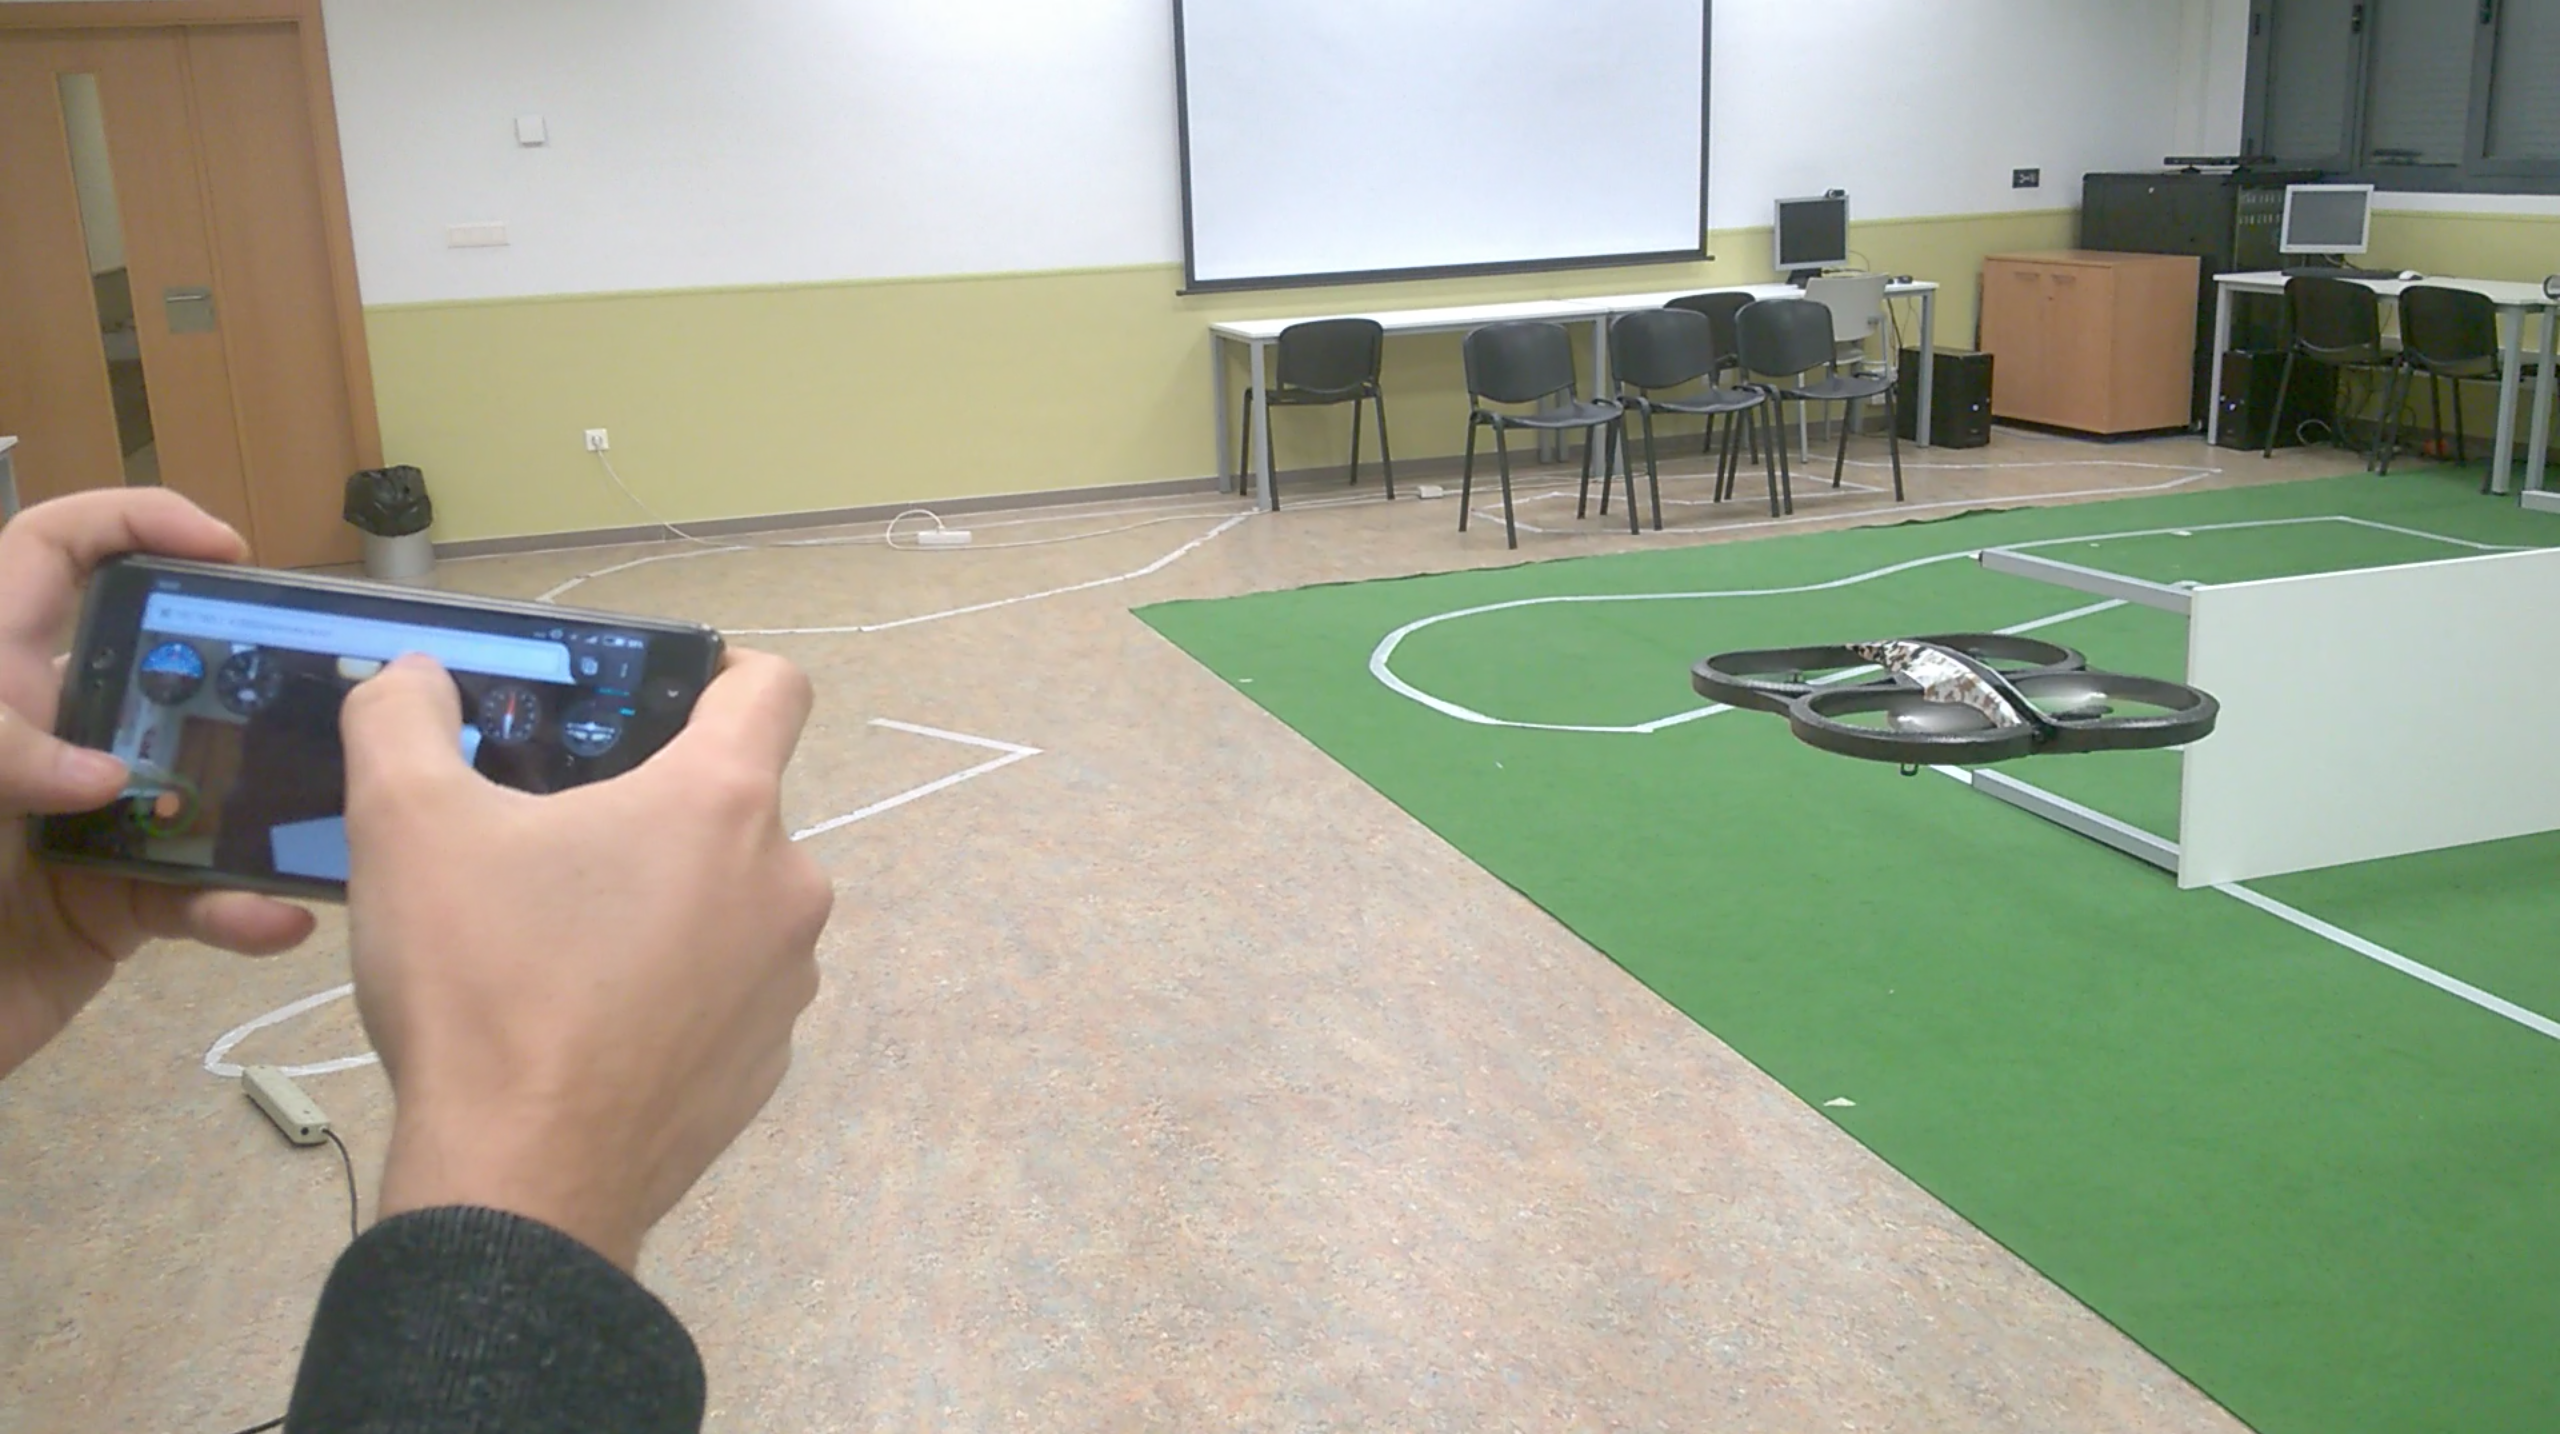
\includegraphics[width=0.9\textwidth]{experimentodronemultidispositivo1}
\caption{Experimento con móvil como par remoto.}
\label{fig:experimentodronemultidispositivo1}
\end{figure}

El segundo experimento es a la inversa, se utiliza un ordenador como par remoto y un dispositivo móvil como par local, encargándose de establecer la conexion con el drone. En este caso las imágenes que se envían son de una de las dos cámaras del móvil, la delantera o la trasera, pudiendo elegir cualquiera de las dos. La figura \ref{fig:experimentodronemultidispositivo2} muestra un momento del experimento que esta recogido en un vídeo en la mediawiki\footnote{\url{http://jderobot.org/Irodmar-tfg#Flying_with_a_mobile_like_Droner_PC}}.\\

\begin{figure}[h!]
\centering
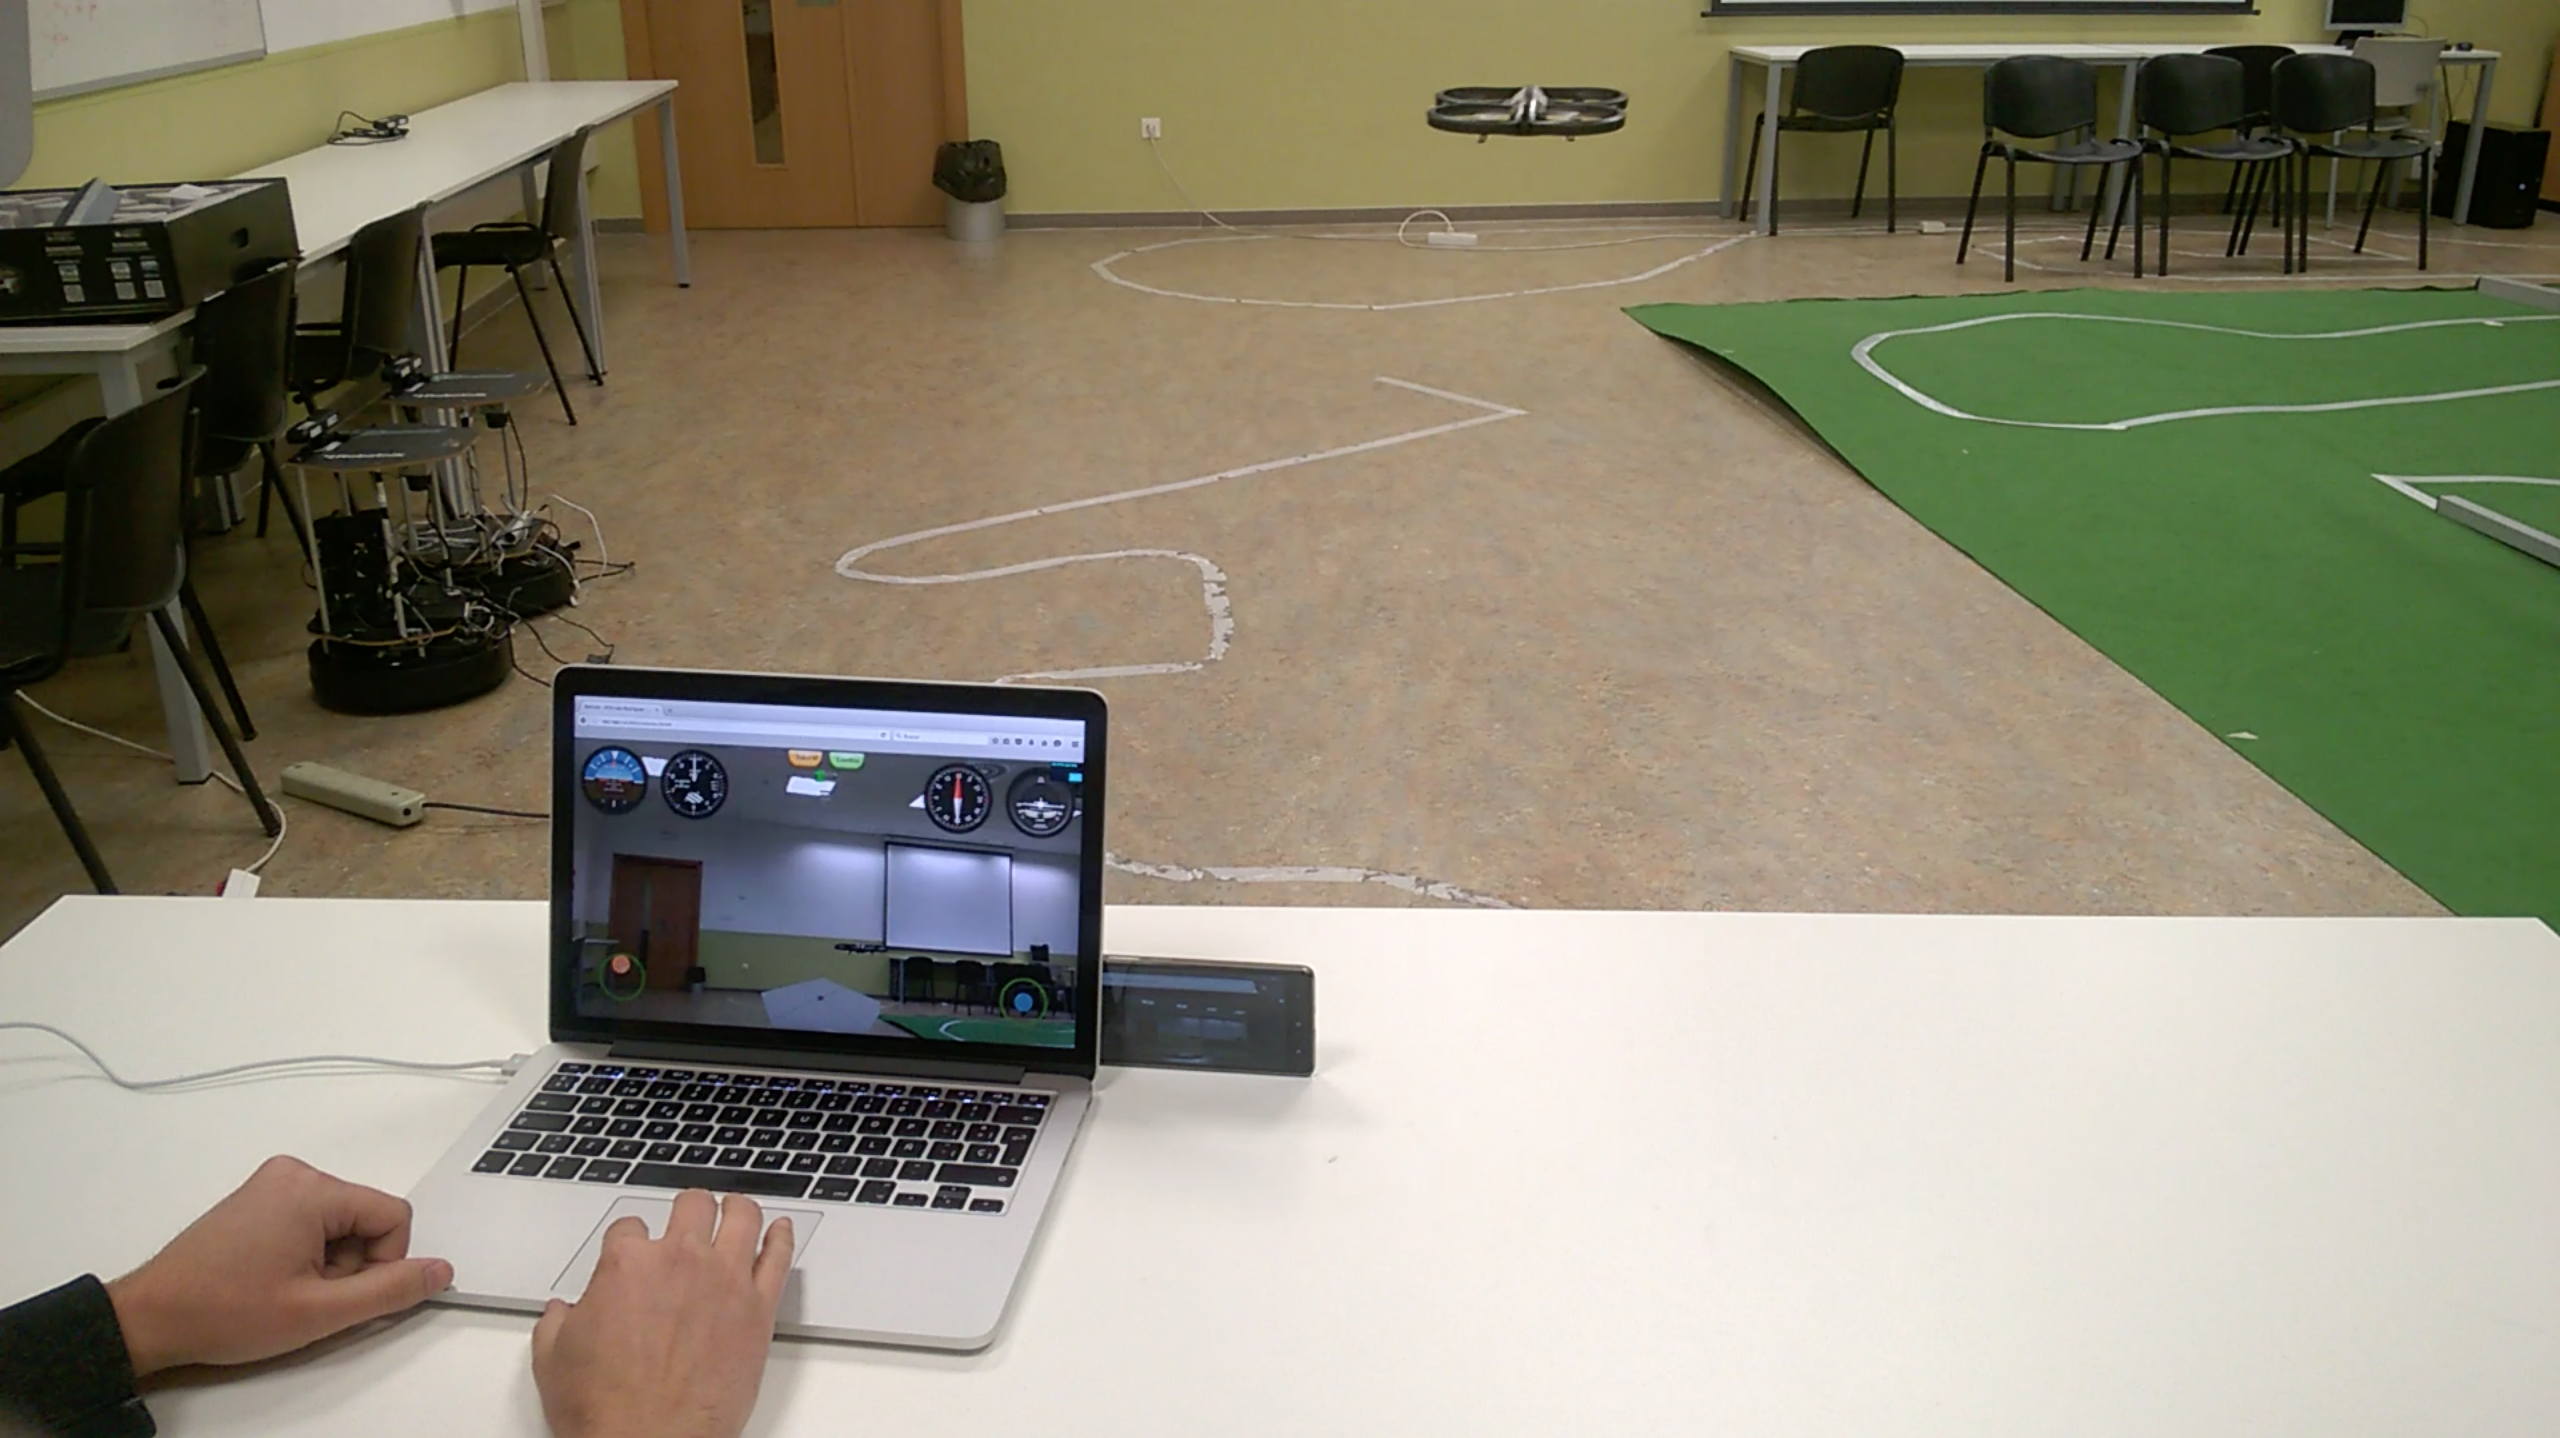
\includegraphics[width=0.9\textwidth]{experimentodronemultidispositivo2}
\caption{Experimento con móvil como par local.}
\label{fig:experimentodronemultidispositivo2}
\end{figure}